\documentclass[journal]{IEEEtran}
\usepackage[a5paper, margin=10mm, onecolumn]{geometry}
\usepackage{lmodern}

\setlength{\headheight}{1cm}
\setlength{\headsep}{0mm}

\usepackage{gvv-book}
\usepackage{gvv}
\usepackage{cite}
\usepackage{amsmath,amssymb,amsfonts,amsthm}
\usepackage{graphicx}
\graphicspath{{./figs/}}
\usepackage{xcolor}
\usepackage{txfonts}
\usepackage{enumitem}
\usepackage{mathtools}
\usepackage{hyperref}
\usepackage{tikz}
\usepackage{tkz-euclide}

\begin{document}

\bibliographystyle{IEEEtran}
\vspace{3cm}

\title{4.13.41}
\author{EE25BTECH11036 - M Chanakya Srinivas}
\maketitle

\renewcommand{\thetable}{\theenumi}
\setlength{\intextsep}{10pt}
\renewcommand\theequation{\arabic{equation}}




\section*{Problem}
Find the area of the parallelogram formed by the lines
\[
y = mx, \quad y = mx + 1, \quad y = nx, \quad y = nx + 1
\]

\section*{Solution}

\subsection*{Step 1: Express the lines in normal form}

The general form of a line is
\begin{align}
\vec{n}^\top\vec{x} = c
\end{align}
where \(\vec{n}\) is the normal vector and \(c\) is the intercept on the normal.

For the given lines,
\begin{align}
y - mx &= 0 \implies \vec{n}_1^\top\vec{x} = 0,\\
y - mx - 1 &= 0 \implies \vec{n}_2^\top\vec{x} = 1,\\
y - nx &= 0 \implies \vec{n}_3^\top\vec{x} = 0,\\
y - nx - 1 &= 0 \implies \vec{n}_4^\top\vec{x} = 1,
\end{align}
where
\begin{align}
\vec{n}_1 = \vec{n}_2 = \myvec{-m \\ 1}, \quad
\vec{n}_3 = \vec{n}_4 = \myvec{-n \\ 1}.
\end{align}

\subsection*{Step 2: Formula for intersection of two lines}

For two lines 
\(\vec{n}_1^\top\vec{x} = c_1\) and \(\vec{n}_2^\top\vec{x} = c_2\),
their intersection point satisfies
\begin{align}
\myvec{\vec{n}_1^\top \\ \vec{n}_2^\top}\vec{x} = \myvec{c_1 \\ c_2}.
\end{align}
Hence,
\begin{align}
\vec{x} = \myvec{\vec{n}_1^\top \\ \vec{n}_2^\top}^{-1} \myvec{c_1 \\ c_2}.
\end{align}

\subsection*{Step 3: Construct the matrix and its inverse}

\begin{align}
\vec{N} = \myvec{-m & 1 \\ -n & 1}, \qquad
\vec{N}^{-1} = \frac{1}{n - m}\myvec{1 & -1 \\ n & -m}.
\end{align}

\subsection*{Step 4: Compute intersection points}

\noindent
\textbf{(i) Intersection of } \(y=mx\) and \(y=nx\):
\begin{align}
\vec{A} &= \vec{N}^{-1}\myvec{0 \\ 0}
= \myvec{0 \\ 0}.
\end{align}

\noindent
\textbf{(ii) Intersection of } \(y=mx+1\) and \(y=nx\):
\begin{align}
\vec{B} &= \vec{N}^{-1}\myvec{1 \\ 0}
= \frac{1}{n - m}\myvec{1 \\ n}.
\end{align}

\noindent
\textbf{(iii) Intersection of } \(y=mx+1\) and \(y=nx+1\):
\begin{align}
\vec{C} &= \vec{N}^{-1}\myvec{1 \\ 1}
= \frac{1}{n - m}\myvec{0 \\ n - m}
= \myvec{0 \\ 1}.
\end{align}

\noindent
\textbf{(iv) Intersection of } \(y=mx\) and \(y=nx+1\):
\begin{align}
\vec{D} &= \vec{N}^{-1}\myvec{0 \\ 1}
= \frac{1}{n - m}\myvec{-1 \\ -m}.
\end{align}

Thus, the four vertices are
\begin{align}
\vec{A} = \myvec{0 \\ 0}, \quad
\vec{B} = \frac{1}{n - m}\myvec{1 \\ n}, \quad
\vec{C} = \myvec{0 \\ 1}, \quad
\vec{D} = \frac{1}{n - m}\myvec{-1 \\ -m}.
\end{align}

\subsection*{Step 5: Find area of the parallelogram}

Two adjacent sides are:
\begin{align}
\vec{B}-\vec{A} &= \frac{1}{n - m}\myvec{1 \\ n},\\
\vec{D}-\vec{A} &= \frac{1}{n - m}\myvec{-1 \\ -m}.
\end{align}

Area of parallelogram is
\begin{align}
\text{Area} &= \abs{(\vec{B}-\vec{A}) \times (\vec{D}-\vec{A})} \\
&= \left| \frac{1}{(n-m)^2} 
\det\myvec{1 & -1 \\ n & -m} \right| \\
&= \frac{|m - n|}{(n - m)^2} = \frac{1}{|m - n|}.
\end{align}

\subsection*{Final Answer}
\begin{align}
\boxed{\text{Area of the parallelogram} = \frac{1}{|m - n|}}
\end{align}

\begin{figure}[h!]
    \centering
    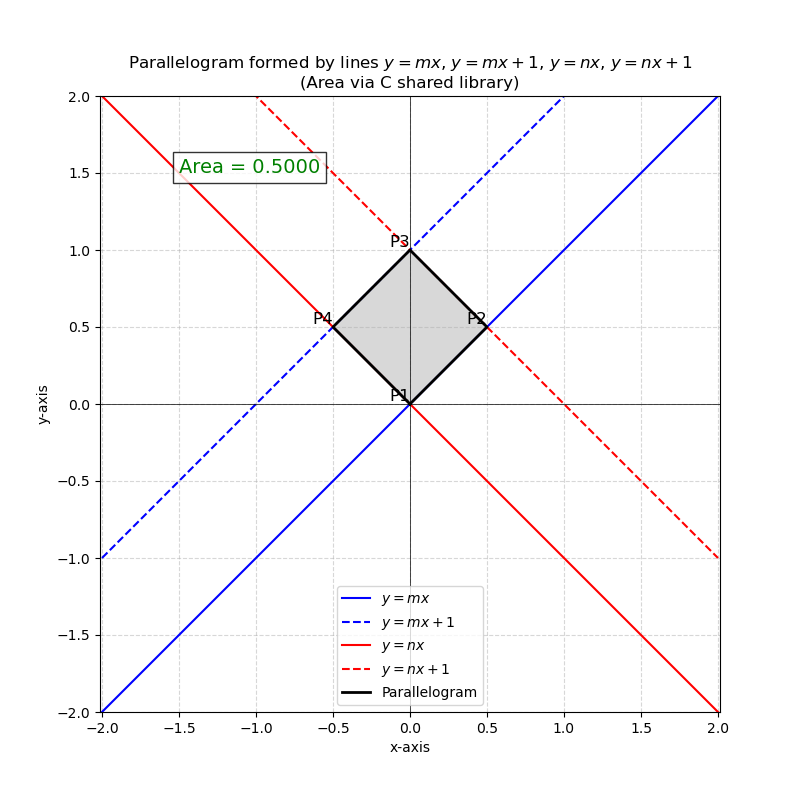
\includegraphics[width=0.9\columnwidth]{figs/Figure_81.png}
    \caption{Parallelogram formed by the given lines.}
\end{figure}

\begin{figure}[h!]
    \centering
    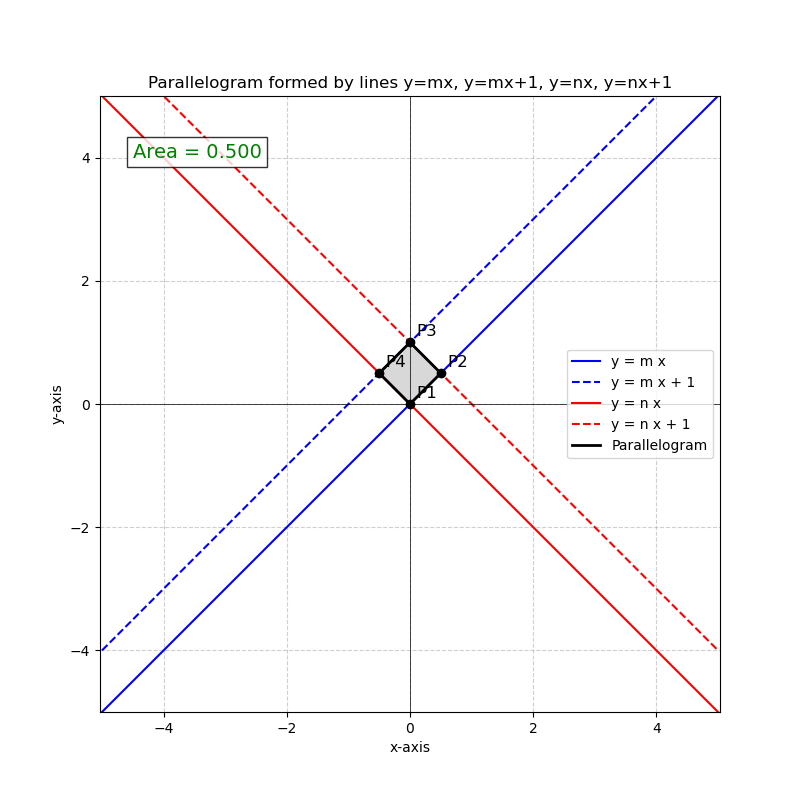
\includegraphics[width=0.9\columnwidth]{figs/fig82.png}
    \caption{Verification of intersection points.}
\end{figure}

\end{document}